% Midterm Results
% Compile with: latexmk -pdf midterm_results.tex
\documentclass[aspectratio=169,11pt]{beamer}

\usepackage[T1]{fontenc}
\usepackage{lmodern}
\usepackage{booktabs}
\usepackage{array}
\usepackage{tikz}
\usetikzlibrary{shapes.geometric,positioning,calc,arrows.meta}
\usepackage{pgfplots}
\pgfplotsset{compat=1.18}
\usepackage[most]{tcolorbox}
\graphicspath{{images/}}

% ---------- Colors ----------
\definecolor{navy}{HTML}{1C2541}
\definecolor{oldred}{HTML}{B22234}   % US flag red, also the accent color
\definecolor{oldblue}{HTML}{3C3B6E}  % US flag blue
\definecolor{ink}{HTML}{2B2B2B}
\definecolor{muted}{HTML}{8A8F98}
\definecolor{paper}{HTML}{FFFFFF}
\definecolor{dem}{HTML}{2E5FA3}      % Democrats
\definecolor{rep}{HTML}{C0392B}      % Republicans
\definecolor{austria}{HTML}{C8102E}  % Austria red, for USA-vs-Austria comparisons

% ---------- Minimal theme ----------
\setbeamertemplate{navigation symbols}{}
\setbeamercolor{normal text}{fg=ink, bg=paper}
\setbeamercolor{structure}{fg=navy}
\setbeamercolor{frametitle}{fg=navy}
\setbeamercolor{alerted text}{fg=oldred}
\setbeamercolor{footnote}{fg=muted}
\setbeamerfont{frametitle}{size=\Large, series=\bfseries}
\setbeamertemplate{itemize item}{\color{oldred}\textbullet}
\setbeamertemplate{itemize subitem}{\color{muted}--}
\setbeamertemplate{enumerate item}{\color{oldred}\insertenumlabel.}
\setbeamersize{text margin left=1.1cm, text margin right=1.1cm}
\hypersetup{colorlinks=true, urlcolor=dem, linkcolor=navy}

\setbeamertemplate{frametitle}{%
  \vspace*{0.5cm}%
  \usebeamerfont{frametitle}\usebeamercolor[fg]{frametitle}\insertframetitle\par
  \vspace{0.15cm}{\color{navy!15}\rule{\textwidth}{0.4pt}}\par}

\setbeamertemplate{footline}{%
  \hfill{\tiny\color{muted}\insertframenumber}\hspace*{0.6cm}\vspace*{0.35cm}}

% Plain divider at the start of each section
\AtBeginSection{%
  \begin{frame}[plain,noframenumbering]
    \centering
    {\LARGE\bfseries\color{navy}\insertsection}\\[0.6em]
    {\color{oldred}\rule{1.5cm}{0.8pt}}
  \end{frame}}

% "Think" question slides: \begin{thinkframe} ... \end{thinkframe}
\newenvironment{thinkframe}{%
  \begin{frame}[plain,noframenumbering,environment=thinkframe]\centering\Large}{\end{frame}}

% ---------- Helpers ----------
% Small grey source line at the bottom of a frame
\newcommand{\source}[1]{%
  \begin{tikzpicture}[remember picture,overlay]
    \node[anchor=south west, font=\tiny, text=muted, text width=0.85\paperwidth, align=left]
      at ($(current page.south west)+(0.6cm,0.25cm)$) {#1};
  \end{tikzpicture}}

% Quote box with a thin red rule on the left; optional arg e.g. [fontupper=\itshape\small]
\newtcolorbox{textquote}[1][]{%
  enhanced, frame hidden, boxrule=0pt, sharp corners,
  colback=navy!4, borderline west={2pt}{0pt}{oldred},
  left=10pt, right=8pt, top=6pt, bottom=6pt, fontupper=\itshape, #1}

% Photo + name + short bio (use inside a column): \candidate{file}{Name}{bio}
\newcommand{\candidate}[3]{%
  \begin{minipage}[t]{\linewidth}\centering
    \includegraphics[height=3.5cm]{#1}\\[0.5em]
    {\large\bfseries\color{navy}#2}\\[0.4em]
    \begin{minipage}{0.9\linewidth}\raggedright\small #3\end{minipage}
  \end{minipage}}

% Big number with a caption (use inside a column): \bignum{color}{91\%}{caption}
\newcommand{\bignum}[3]{%
  \begin{minipage}[t]{\linewidth}\centering
    {\fontsize{34}{38}\selectfont\bfseries\color{#1}#2}\\[0.3em]
    {\small #3}
  \end{minipage}}

% US flag drawn in TikZ (hoist height = #1), e.g. \usflag{3cm}
\newcommand{\usflag}[1]{%
  \begin{tikzpicture}[x=#1, y=#1]
    \def\fly{1.9}
    \foreach \i in {0,...,12} {
      \pgfmathsetmacro{\c}{mod(\i,2)==0 ? 1 : 0}
      \ifdim\c pt=1pt
        \fill[oldred] (0,{1-(\i+1)/13}) rectangle (\fly,{1-\i/13});
      \else
        \fill[white] (0,{1-(\i+1)/13}) rectangle (\fly,{1-\i/13});
      \fi
    }
    \def\cw{0.76} \def\ch{0.5385}
    \fill[oldblue] (0,{1-\ch}) rectangle (\cw,1);
    \foreach \r in {1,...,9} {
      \pgfmathsetmacro{\isodd}{mod(\r,2)}
      \ifdim\isodd pt=1pt
        \foreach \k in {0,...,5}
          \node[star, star points=5, star point ratio=2.618, fill=white, inner sep=0pt,
                minimum size=0.0616*#1] at ({(2*\k+1)*\cw/12},{1-\r*\ch/10}) {};
      \else
        \foreach \k in {0,...,4}
          \node[star, star points=5, star point ratio=2.618, fill=white, inner sep=0pt,
                minimum size=0.0616*#1] at ({(2*\k+2)*\cw/12},{1-\r*\ch/10}) {};
      \fi
    }
    \draw[ink!30, line width=0.3pt] (0,0) rectangle (\fly,1);
  \end{tikzpicture}}

% Agree/disagree spectrum for "spectrum game" activities
\newcommand{\spectrum}{%
  
\begin{tikzpicture}
    \shade[left color=oldblue, right color=oldred, rounded corners=2pt] (0,0) rectangle (11,0.18);
    \node[anchor=north, font=\small, text=oldblue] at (0,-0.15) {Strongly disagree};
    \node[anchor=north, font=\small, text=muted] at (5.5,-0.15) {Neutral};
    \node[anchor=north, font=\small, text=oldred] at (11,-0.15) {Strongly agree};
    \fill[paper, draw=muted] (5.5,0.09) circle (2.5pt);
  \end{tikzpicture}}

% One statement per slide: \statement{number}{total}{text}
\newcommand{\statement}[3]{%
  \begin{frame}[plain]
    \vfill
    \begin{center}
      {\small\color{muted}Statement #1 of #2}\\[1.2em]
      {\LARGE\bfseries #3}
    \end{center}
    \vfill
    \begin{center}\spectrum\end{center}
    \vspace{1.2cm}
  \end{frame}}


% State profile: \profile{Title}{photo}{locator}{bullets}{question}{answer}{source}
\newcommand{\profile}[7]{%
  \begin{frame}{#1}
    \begin{columns}[c]
      \begin{column}{0.4\textwidth}
        \begin{itemize}\setlength{\itemsep}{0.7em}
          #4
        \end{itemize}
        \vspace{0.9em}
        {\bfseries\color{navy}#5}\\[0.4em]
        \visible<2>{{\LARGE\bfseries\color{oldred}#6}}
      \end{column}
      \begin{column}{0.55\textwidth}
        \centering
        \begin{tikzpicture}
          \node[inner sep=0pt] (ph) {\includegraphics[width=\linewidth]{#2}};
          \node[anchor=south east, inner sep=2pt, fill=white] at (ph.south east)
            {\includegraphics[width=2.5cm]{#3}};
        \end{tikzpicture}
      \end{column}
    \end{columns}
    \source{#7}
  \end{frame}}

% Candidate face: \face{photo}{Name (D)}{tag}{color}
\newcommand{\face}[4]{%
  \begin{minipage}[t]{4.6cm}\centering
    \includegraphics[height=2.7cm]{#1}\\[0.3em]
    {\bfseries\color{#4}#2}\\[0.1em]
    {\small\color{muted}#3}
  \end{minipage}}

% Grey silhouette the same size as a face photo
\newcommand{\silhouette}{%
  
\begin{tikzpicture}
    \fill[navy!8] (0,0) rectangle (2.64cm,3.3cm);
    \begin{scope}
      \clip (0,0) rectangle (2.64cm,3.3cm);
      \fill[muted!70] (1.32cm,2.05cm) circle (0.62cm);
      \fill[muted!70] (1.32cm,-0.25cm) ellipse (1.15cm and 1.55cm);
    \end{scope}
    \node[font=\Huge\bfseries, text=white] at (1.32cm,2.05cm) {?};
  \end{tikzpicture}}

% Result line: \result{Winner 53\%}{Loser 47\%}
\newcommand{\result}[2]{{\LARGE\bfseries\color{dem}#1}\qquad{\Large\color{rep}#2}}
\newcommand{\issues}[1]{{\small\textbf{Top issues:} #1}}

% Photo tile for the cheat sheet: \tile{photo}{State}{words}
\newcommand{\tile}[3]{%
  \begin{minipage}[t]{4.1cm}\centering
    \includegraphics[width=3.3cm]{#1}\\[0.2em]
    {\small\bfseries\color{navy}#2}\\[-0.1em]
    {\footnotesize #3}
  \end{minipage}}

% Scenario slide: \scenario{Title}{line 1}{line 2}{question}
\newcommand{\scenario}[4]{%
  \begin{frame}{#1}
    \centering
    \vspace{0.6em}
    {\Large #2}\\[0.7em]
    {\Large #3}\\[1.4em]
    {\LARGE\bfseries\color{oldred}#4}
  \end{frame}}

% US map with six states in red; #1 = labels drawn on top (coordinates as fractions of the map)
\newcommand{\usmap}[1]{%
  \begin{tikzpicture}[x=8.6cm, y=-5.32cm]
    \node[anchor=north west, inner sep=0pt] at (0,0) {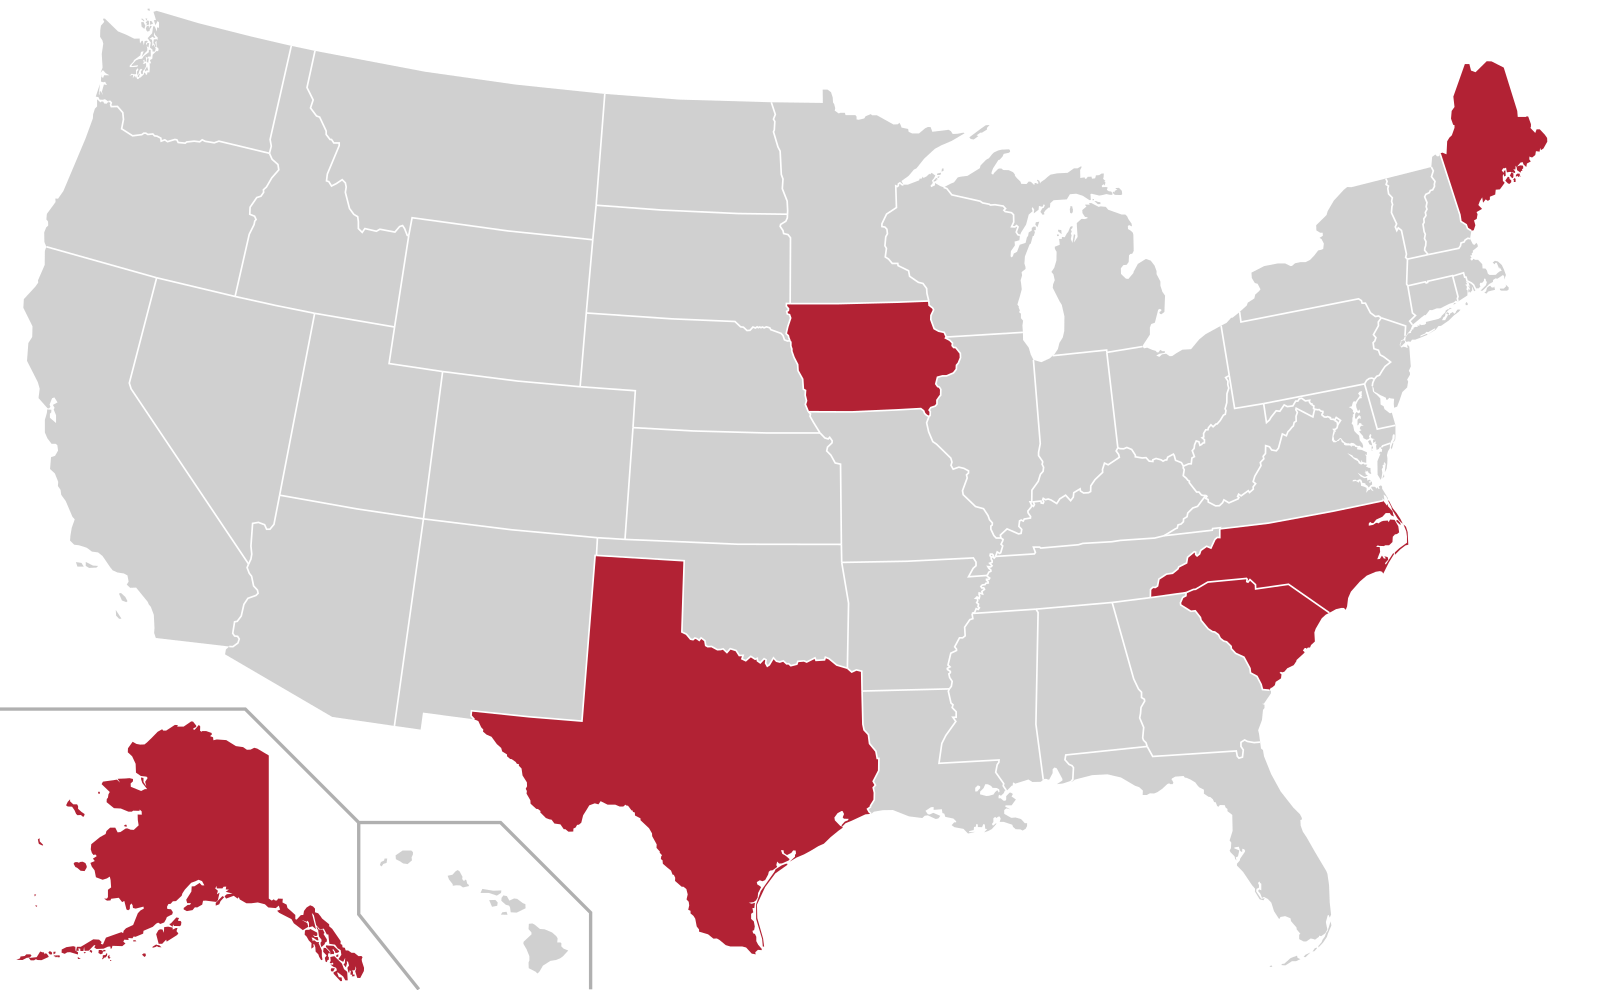
\includegraphics[width=8.6cm]{usmap.png}};
    #1
  \end{tikzpicture}}

\begin{document}

% ---------- Title slide ----------
\begin{frame}[plain]
  \begin{columns}[c]
    \begin{column}{0.5\textwidth}
      {\fontsize{30}{34}\selectfont\bfseries\color{navy} Midterm\\Results}\\[0.8em]
      {\Large\color{muted} Six states that changed the Senate}\\[0.6em]
      {\color{oldred}\rule{3cm}{1.5pt}}
    \end{column}
    \begin{column}{0.45\textwidth}
      \centering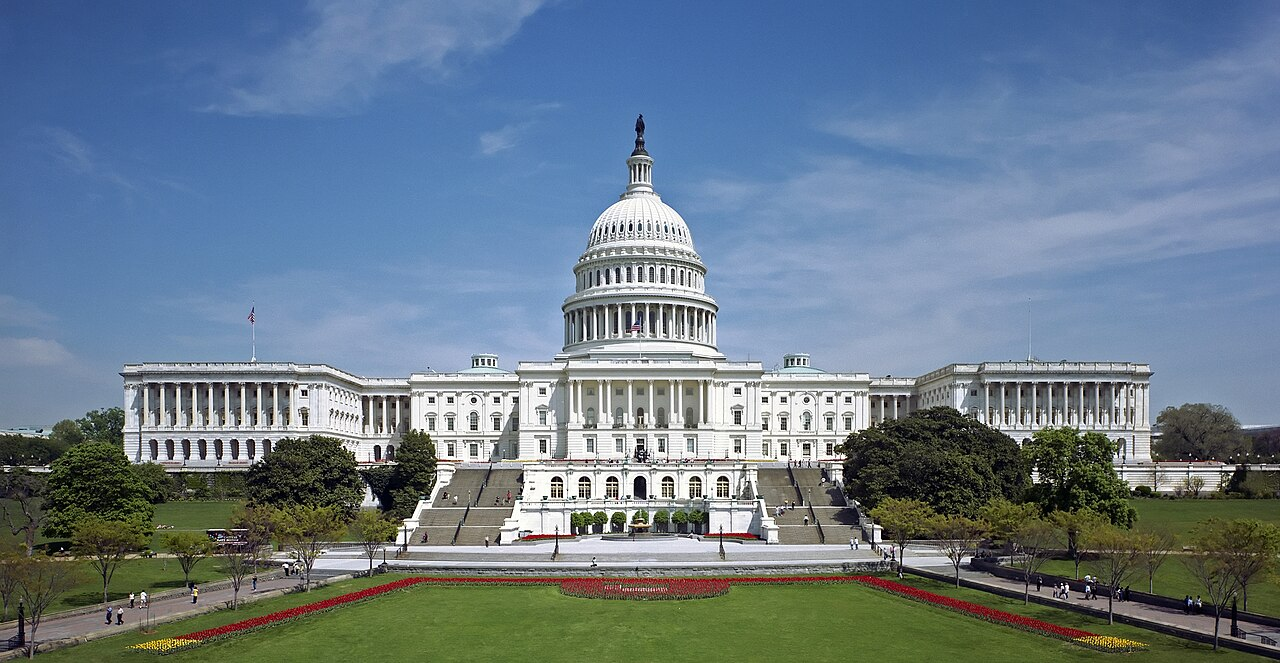
\includegraphics[width=\linewidth]{capitol.jpg}
    \end{column}
  \end{columns}
\end{frame}

% =====================================================================
\section{Warm-up}

\begin{frame}{Where are these states?}
  \begin{columns}[c]
    \begin{column}{0.62\textwidth}
      \centering
      \usmap{
        \node[font=\bfseries\large, text=white] at (0.42,0.74) {A};
        \node[font=\bfseries\large, text=white] at (0.932,0.16) {B};
        \node[font=\bfseries\large, text=white] at (0.115,0.83) {C};
        \node[font=\bfseries\large, text=navy] (d) at (0.87,0.70) {D};
        \draw[navy, line width=0.5pt] (d) -- (0.795,0.645);
        \node[font=\bfseries\large, text=white] at (0.546,0.36) {E};
        \node[font=\bfseries\large, text=white] at (0.80,0.555) {F};
      }
    \end{column}
    \begin{column}{0.32\textwidth}
      \begin{itemize}\setlength{\itemsep}{0.5em}
        \item Alaska
        \item Iowa
        \item Maine
        \item North Carolina
        \item South Carolina
        \item Texas
      \end{itemize}
      \vspace{0.6em}
      {\bfseries\color{oldred}Match the letters}
    \end{column}
  \end{columns}
\end{frame}

\begin{frame}{The six states}
  \centering
  \usmap{
    \node[font=\bfseries\small, text=white] at (0.42,0.74) {Texas};
    \node[font=\bfseries\small, text=navy, anchor=east] at (0.905,0.10) {Maine};
    \node[font=\bfseries\small, text=white] at (0.115,0.83) {Alaska};
    \node[font=\bfseries\small, text=navy, anchor=west] (d) at (0.84,0.71) {South Carolina};
    \draw[navy, line width=0.5pt] (d.west) -- (0.795,0.645);
    \node[font=\bfseries\small, text=white] at (0.546,0.36) {Iowa};
    \node[font=\bfseries\small, text=navy, anchor=west] (f) at (0.90,0.52) {North Carolina};
    \draw[navy, line width=0.5pt] (f.west) -- (0.83,0.55);
  }\\[0.3em]
  All six: a \alert{Republican} seat
\end{frame}

\begin{frame}{The game}
  \centering
  \vspace{0.5em}
  {\Large When did each state last elect a \textbf{\color{dem}Democratic} senator?}\\[1.4em]
  {\Large Guess: \alert{more} or \alert{less} recently than the last state?}
\end{frame}

% =====================================================================
\section{State by State}

\profile{Maine}{maine.jpg}{loc_me.png}{
  \item \alert{1.4 million} people
  \item The \alert{oldest} state
  \item Rural, 90\% white
  \item Never voted for Trump statewide
}{Guess the year}{1988}{Source: US Census Bureau. Photo: Bd2media, CC BY-SA 4.0.}

\begin{frame}{Maine: the race}
  \centering
  \face{jackson.jpg}{Troy Jackson (D)}{logger}{dem}\hspace{0.4cm}%
  \face{collins.jpg}{Susan Collins (R)}{senator since 1997}{rep}\\[0.6em]
  \issues{health care, pensions}\\[0.5em]
  \result{Jackson 53\%}{Collins 47\%}
  \source{As of Nov.\ 12, unofficial (AP). Issues: CBS exit poll.}
\end{frame}

\begin{frame}{Why not Platner?}
  \begin{columns}[c]
    \begin{column}{0.6\textwidth}
      \begin{itemize}\setlength{\itemsep}{0.6em}
        \item Won the Democratic primary
        \item Old Reddit posts found:
          \begin{itemize}
            \item ``all cops are bastards''
            \item joined the Marines ``to have an adventure and kill some people''
          \end{itemize}
        \item July: accused of rape (he denies it)
        \item He quit; Democrats chose Jackson
      \end{itemize}
    \end{column}
    \begin{column}{0.32\textwidth}
      \centering
      
\includegraphics[height=4cm]{platner.jpg}\\[0.3em]
      {\small\bfseries\color{navy}Graham Platner}
    \end{column}
  \end{columns}
  \source{Source: CNN; Politico. Photo: MAINEiac4434, CC BY-SA 4.0.}
\end{frame}

\profile{North Carolina}{nc.jpg}{loc_nc.png}{
  \item \alert{11 million} people, growing fast
  \item \alert{1 in 5} is Black
  \item Banks, universities, tech
  \item A \alert{swing state}: Obama 2008, then Trump
}{More or less recently than Maine?}{More: 2008}{Source: US Census Bureau. Photo: Charlotte (brandon walker, CC0).}

\begin{frame}{North Carolina: the race}
  \centering
  \face{cooper.jpg}{Roy Cooper (D)}{former governor}{dem}\hspace{0.4cm}%
  \face{whatley.jpg}{Michael Whatley (R)}{Trump's party chairman}{rep}\\[0.6em]
  \issues{health care, Cooper's record as governor}\\[0.5em]
  \result{Cooper 59\%}{Whatley 39\%}
  \source{As of Nov.\ 12, unofficial (AP). Issues: Searchlight poll. Photos: NCDOT, CC BY 2.0; Gage Skidmore, CC BY-SA 2.0.}
\end{frame}

\profile{Texas}{texas.jpg}{loc_tx.png}{
  \item \alert{31 million} people
  \item \alert{40\% Hispanic}
  \item Long border with Mexico
  \item Issues: \alert{immigration}, the economy
}{More or less recently than North Carolina?}{Less: 1988}{Source: US Census Bureau. Photo: border wall in the Rio Grande Valley (US Customs and Border Protection).}

\begin{frame}{Texas: the race}
  \centering
  \face{talarico.jpg}{James Talarico (D)}{former teacher}{dem}\hspace{0.4cm}%
  \face{paxton.jpg}{Ken Paxton (R)}{Texas Attorney General}{rep}\\[0.6em]
  \issues{immigration, the border}\\[0.5em]
  \result{Talarico 55\%}{Paxton 43\%}
  \source{As of Nov.\ 12, unofficial (AP). Issues: Searchlight poll. Photos: Antonioaesparza, CC BY-SA 4.0; Gage Skidmore, CC BY-SA 2.0.}
\end{frame}

\profile{Iowa}{iowa.jpg}{loc_ia.png}{
  \item \alert{3 million} people
  \item Mostly white farmers
  \item Number one for \alert{corn} and \alert{pork}
  \item \alert{Diesel prices} matter
}{More or less recently than Texas?}{More: 2008}{Source: US Census Bureau; USDA. Photo: inkknife\_2000, CC BY-SA 2.0.}

\begin{frame}{Iowa: the race}
  \centering
  \face{turek.jpg}{Josh Turek (D)}{Paralympic champion}{dem}\hspace{0.4cm}%
  \face{hinson.jpg}{Ashley Hinson (R)}{congresswoman}{rep}\\[0.6em]
  \issues{farm incomes, diesel prices}\\[0.5em]
  \result{Turek 51\%}{Hinson 46\%}
  \source{As of Nov.\ 12, unofficial (AP). Photos: Iowa General Assembly; Office of Rep.\ Hinson.}
\end{frame}

\profile{South Carolina}{sc.jpg}{loc_sc.png}{
  \item \alert{5.5 million} people
  \item \alert{26\% Black} (Texas: 13\%)
  \item Religious and conservative
  \item Republican since 1980
}{More or less recently than Iowa?}{Less: 1998}{Source: US Census Bureau. Photo: Rainbow Row, Charleston (Thomson200, CC0).}

\begin{frame}{South Carolina: the race}
  \centering
  \face{andrews.jpg}{Annie Andrews (D)}{children's doctor}{dem}\hspace{0.4cm}%
  \face{dgraham.jpg}{Darline Graham (R)}{Lindsey Graham's sister}{rep}\\[0.4em]
  {\small Senator Lindsey Graham died in July}\\[0.1em]
  \issues{Graham's lack of experience}\\[0.4em]
  \result{Andrews 51\%}{Graham 47\%}
  \source{As of Nov.\ 12, unofficial (AP). Photos: Jeremy Lauten, CC0; US Senate.}
\end{frame}

\profile{Alaska}{alaska.jpg}{loc_ak.png}{
  \item Only \alert{740,000} people
  \item The \alert{biggest} state
  \item \alert{1 in 5} is Alaska Native
  \item Oil pays for everything
}{More or less recently than South Carolina?}{More: 2008}{Source: US Census Bureau. Photo: Trans-Alaska Pipeline (Luca Galuzzi, CC BY-SA 2.5).}

\begin{frame}{Alaska: the race}
  \begin{columns}[c]
    \begin{column}{0.66\textwidth}
      \centering
      \begin{minipage}[t]{2.9cm}\centering
        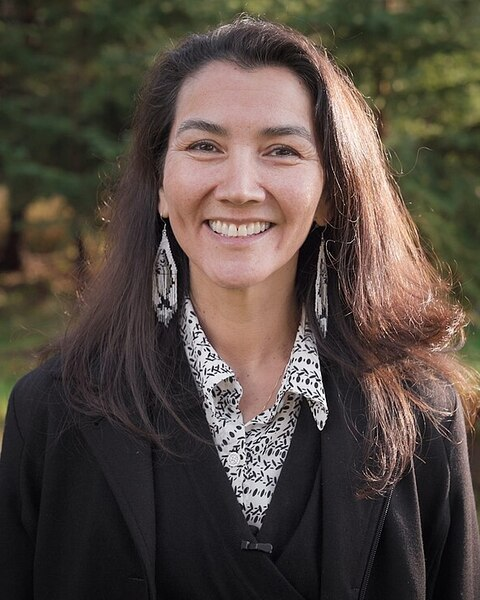
\includegraphics[height=3.3cm]{peltola.jpg}\\[0.3em]
        {\small\bfseries\color{dem}Mary Peltola (D)}
      \end{minipage}\hfill
      \begin{minipage}[t]{2.9cm}\centering
        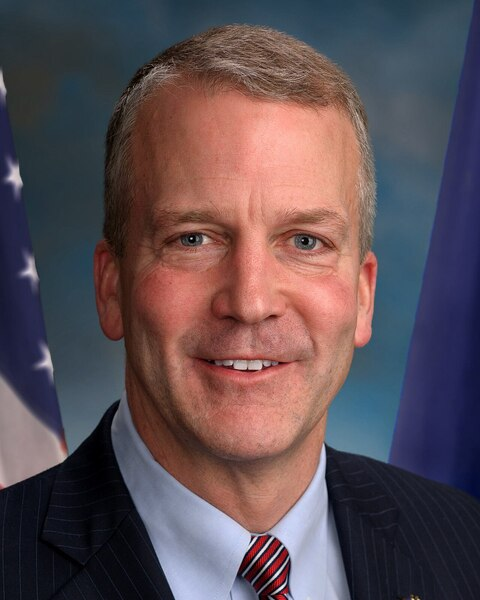
\includegraphics[height=3.3cm]{sullivan.jpg}\\[0.3em]
        {\small\bfseries\color{rep}Dan Sullivan (R)}\\[-0.1em]
        {\footnotesize\color{muted}senator}
      \end{minipage}\hfill
      \begin{minipage}[t]{2.9cm}\centering
        \silhouette\\[0.3em]
        {\small\bfseries\color{ink}Dan Sullivan}\\[-0.1em]
        {\footnotesize\color{muted}retired teacher}
      \end{minipage}
    \end{column}
    \begin{column}{0.32\textwidth}
      \begin{itemize}\setlength{\itemsep}{0.7em}
        \item \textbf{Top issues:} oil prices, fishing
        \item \alert{Two} Dan Sullivans on the ballot
        \item \alert{Still counting:} Peltola ahead by 2,500 votes
        \item Final count: November 18
      \end{itemize}
    \end{column}
  \end{columns}
  \source{Source: Alaska Beacon, Nov.\ 9. Not final. Photos: US House of Representatives; US Senate.}
\end{frame}

\begin{frame}{When did they last elect a Democrat?}
  \centering
  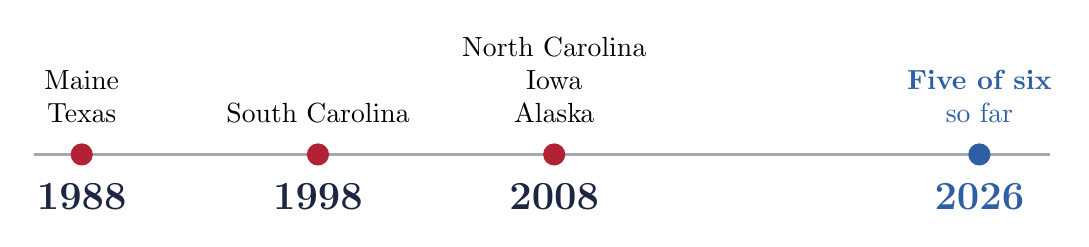
\begin{tikzpicture}[x=0.3cm, y=1cm]
    \draw[navy!40, line width=1.2pt] (-2,0) -- (41,0);
    \foreach \x in {0,10,20} \fill[oldred] (\x,0) circle (4pt);
    \fill[dem] (38,0) circle (4pt);
    \node[font=\bfseries\Large, text=navy, below=7pt] at (0,0) {1988};
    \node[font=\bfseries\Large, text=navy, below=7pt] at (10,0) {1998};
    \node[font=\bfseries\Large, text=navy, below=7pt] at (20,0) {2008};
    \node[font=\bfseries\Large, text=dem, below=7pt] at (38,0) {2026};
    \node[align=center, above=8pt] at (0,0) {Maine\\Texas};
    \node[align=center, above=8pt] at (10,0) {South Carolina};
    \node[align=center, above=8pt] at (20,0) {North Carolina\\Iowa\\Alaska};
    \node[align=center, above=8pt, text=dem] at (38,0) {\textbf{Five of six}\\so far};
  \end{tikzpicture}
\end{frame}

\begin{frame}{The new Senate}
  \centering
  
\begin{tikzpicture}[x=0.125cm, y=1cm]
    \fill[dem] (0,0) rectangle (55,0.9);
    \fill[muted!60] (55,0) rectangle (56,0.9);
    \fill[rep] (56,0) rectangle (100,0.9);
    \node[font=\bfseries\Large, text=white] at (27.5,0.45) {Democrats 55};
    \node[font=\bfseries\Large, text=white] at (78,0.45) {Republicans 44};
    \draw[ink, line width=0.8pt, dashed] (50.5,-0.25) -- (50.5,1.15);
    \node[font=\scriptsize, text=ink, anchor=south] at (50.5,1.15) {51 for a majority};
    \node[font=\scriptsize, text=muted, anchor=north] at (55.5,-0.05) {1 undecided};
  \end{tikzpicture}
  \vspace{0.8em}
  \begin{itemize}\setlength{\itemsep}{0.6em}
    \item Before: Republicans 53, Democrats 47
    \item Democrats flipped \alert{8 seats}
    \item Number one issue everywhere: the \alert{cost of living}
  \end{itemize}
  \source{Source: AP; CBS News, as of Nov.\ 12. The 55 includes two independents. Issue: NBC and CBS exit polls.}
\end{frame}

% =====================================================================
\section{Output Practice}

\begin{frame}{You are the new senator}
  \begin{itemize}\setlength{\itemsep}{1em}
    \item Each table is one state
    \item Something goes wrong in America
    \item Your state votes: \alert{yes} or \alert{no}?
    \item Tell us why
  \end{itemize}
\end{frame}

\begin{frame}{Your state at a glance}
  \centering
  \tile{tile_maine.jpg}{Maine}{old, rural}\hfill
  \tile{tile_nc.jpg}{North Carolina}{swing state, growing}\hfill
  \tile{tile_texas.jpg}{Texas}{border, oil, 40\% Hispanic}\\[0.7em]
  \tile{tile_iowa.jpg}{Iowa}{farmers, diesel}\hfill
  \tile{tile_sc.jpg}{South Carolina}{conservative, 26\% Black}\hfill
  \tile{tile_alaska.jpg}{Alaska}{oil pays for everything}
\end{frame}

\scenario{Scenario 1: the fire}
  {A huge fire destroys \alert{half of America's oil}}
  {Petrol now costs three times as much}
  {Do you vote to buy oil from Russia?}

\scenario{Scenario 2: the robots}
  {A company invents a \alert{robot farmer}}
  {Food gets cheaper. Farm workers lose their jobs}
  {Do you vote to ban the robot?}

\scenario{Scenario 3: the birthday}
  {Americans now live to \alert{100}}
  {The pension money is running out}
  {Do you vote to raise the retirement age to 80?}

\end{document}
